\documentclass[border=1pt,multi,tikz]{standalone}
\usetikzlibrary{arrows}
\usepackage[utf8]{inputenc}
\usepackage{mathpazo}
\usepackage[euler-digits,euler-hat-accent]{eulervm}
\usepackage[T1]{fontenc}
\usepackage[spanish]{babel}
\usepackage{amsmath,amsfonts,amssymb}
\usepackage{wasysym}
\usepackage[separate-uncertainty=true,multi-part-units=single,binary-units]{siunitx}
\usepackage{graphics}

\begin{document}
\thispagestyle{empty}

\begin{tikzpicture}[every edge quotes/.append style={auto, text=blue} scale=1.0]
	\pgfmathsetmacro{\cubex}{1.25}
	\pgfmathsetmacro{\cubey}{0.65}
	\pgfmathsetmacro{\cubez}{10}
	\draw [every edge/.append style={densely dashed, opacity=.5},fill=gray,opacity=0.25]
(0,0,0) coordinate (o) -- ++(-\cubex,0,0) coordinate (a) -- ++(0,-\cubey,0) coordinate (b) edge coordinate [pos=1] (g) ++(0,0,-\cubez)  -- ++(\cubex,0,0) coordinate (c) -- cycle
(o) -- ++(0,0,-\cubez) coordinate (d) -- ++(0,-\cubey,0) coordinate (e) edge (g) -- (c) -- cycle
(o) -- (a) -- ++(0,0,-\cubez) coordinate (f) edge (g) -- (d) -- cycle;
	\path [every edge/.append style={|-|}]
    (b) +(0,-10pt) coordinate (b1) edge node[below] {\SI{2.5}{\cm}} (b1 -| c)
    (b) +(-10pt,0) coordinate (b2) edge node[left] {\SI{1.3}{\cm}} (b2 |- a)
    (a) +(-5.0pt,5.0pt) coordinate (a2) edge node[left=10pt] {\SI{300}{\cm}} ([xshift=-5.0pt,yshift=5.0pt]f);

	\draw[very thick](-0.625,-0.325) circle (0.05)	;
	\draw[stealth-,thick] (-0.525,-0.325) -- (1.75cm,-0.325) node[right=5pt] {$\diameter=$\SI{1.8}{\mm}};
	\draw[green,very thick](-0.625,-0.325) --++ (-2.0,-2.0);
	\node[inner sep=0pt] (spectra) at (9,1)
    {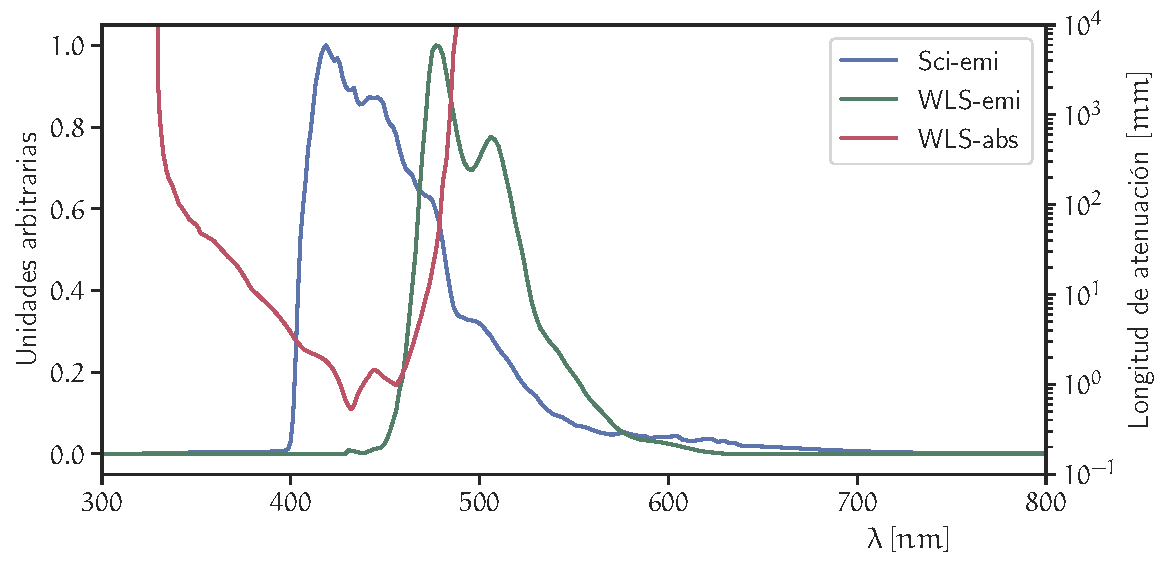
\includegraphics[width=0.8\textwidth]{scibar-optics.pdf}};
\end{tikzpicture}

\end{document}
